\documentclass[12pt,-letter paper]{article}      
\usepackage{siunitx}                             
\usepackage{setspace}
\usepackage{gensymb}                             
\usepackage{xcolor}                              
\usepackage{caption}
%\usepackage{subcaption}
\doublespacing                                   
\singlespacing                                   
\usepackage[none]{hyphenat}
\usepackage{amssymb}
\usepackage{relsize}
\usepackage[cmex10]{amsmath}
\usepackage{mathtools}
\usepackage{amsmath}                            
\usepackage{commath}                             
\usepackage{amsthm}
\interdisplaylinepenalty=2500
%\savesymbol{iint}
\usepackage{txfonts}                             
%\restoresymbol{TXF}{iint}                       
\usepackage{wasysym}                             
\usepackage{amsthm}
\usepackage{mathrsfs}                            
\usepackage{txfonts}                             
\let\vec\mathbf{}
\usepackage{stfloats}
\usepackage{float}
\usepackage{cite}
\usepackage{cases}                               
\usepackage{subfig}                              
%\usepackage{xtab}
\usepackage{longtable}
\usepackage{multirow}
%\usepackage{algorithm}
\usepackage{amssymb}
%\usepackage{algpseudocode}
\usepackage{enumitem}
\usepackage{mathtools}
%\usepackage{eenrc}
%\usepackage[framemethod=tikz]{mdframed}         
\usepackage{listings}                            
%\usepackage{listings}
\usepackage[latin1]{inputenc}
%%\usepackage{color}{
%%\usepackage{lscape}
\usepackage{textcomp}
\usepackage{titling}
\usepackage{hyperref}
%\usepackage{fulbigskip}
\usepackage{tikz}
\usepackage{graphicx}                            
\lstset{
  frame=single,
  breaklines=true
}
\let\vec\mathbf{}
\usepackage{enumitem}                           
\usepackage{graphicx}                            
\usepackage{siunitx}
\let\vec\mathbf{}                                
\usepackage{enumitem}
\usepackage{graphicx}
\usepackage{enumitem}
\usepackage{tfrupee}
\usepackage{amsmath}
\usepackage{amssymb}
\usepackage{mwe} % for blindtext and example-image-a in example
\usepackage{wrapfig}
\title{CIRCLES}
\author{Sujith 02}
\date{December 2023}
\begin{document}
\maketitle
\begin{enumerate}
\item In \figref{fig:circ.jpg}, from an external point $P$,two tangents $PQ$ and $PR$ are drawn to a circle of radius $4cm$ with centre $O$. If $\angle QPR=90\degree$ ,then length of $PQ$ is 
\begin{enumerate}[label=(\Alph*)]
\item $3cm$
\item $4cm$
\item $2cm$
\item $2\sqrt{2}cm$
\begin{figure}[H]
\centering
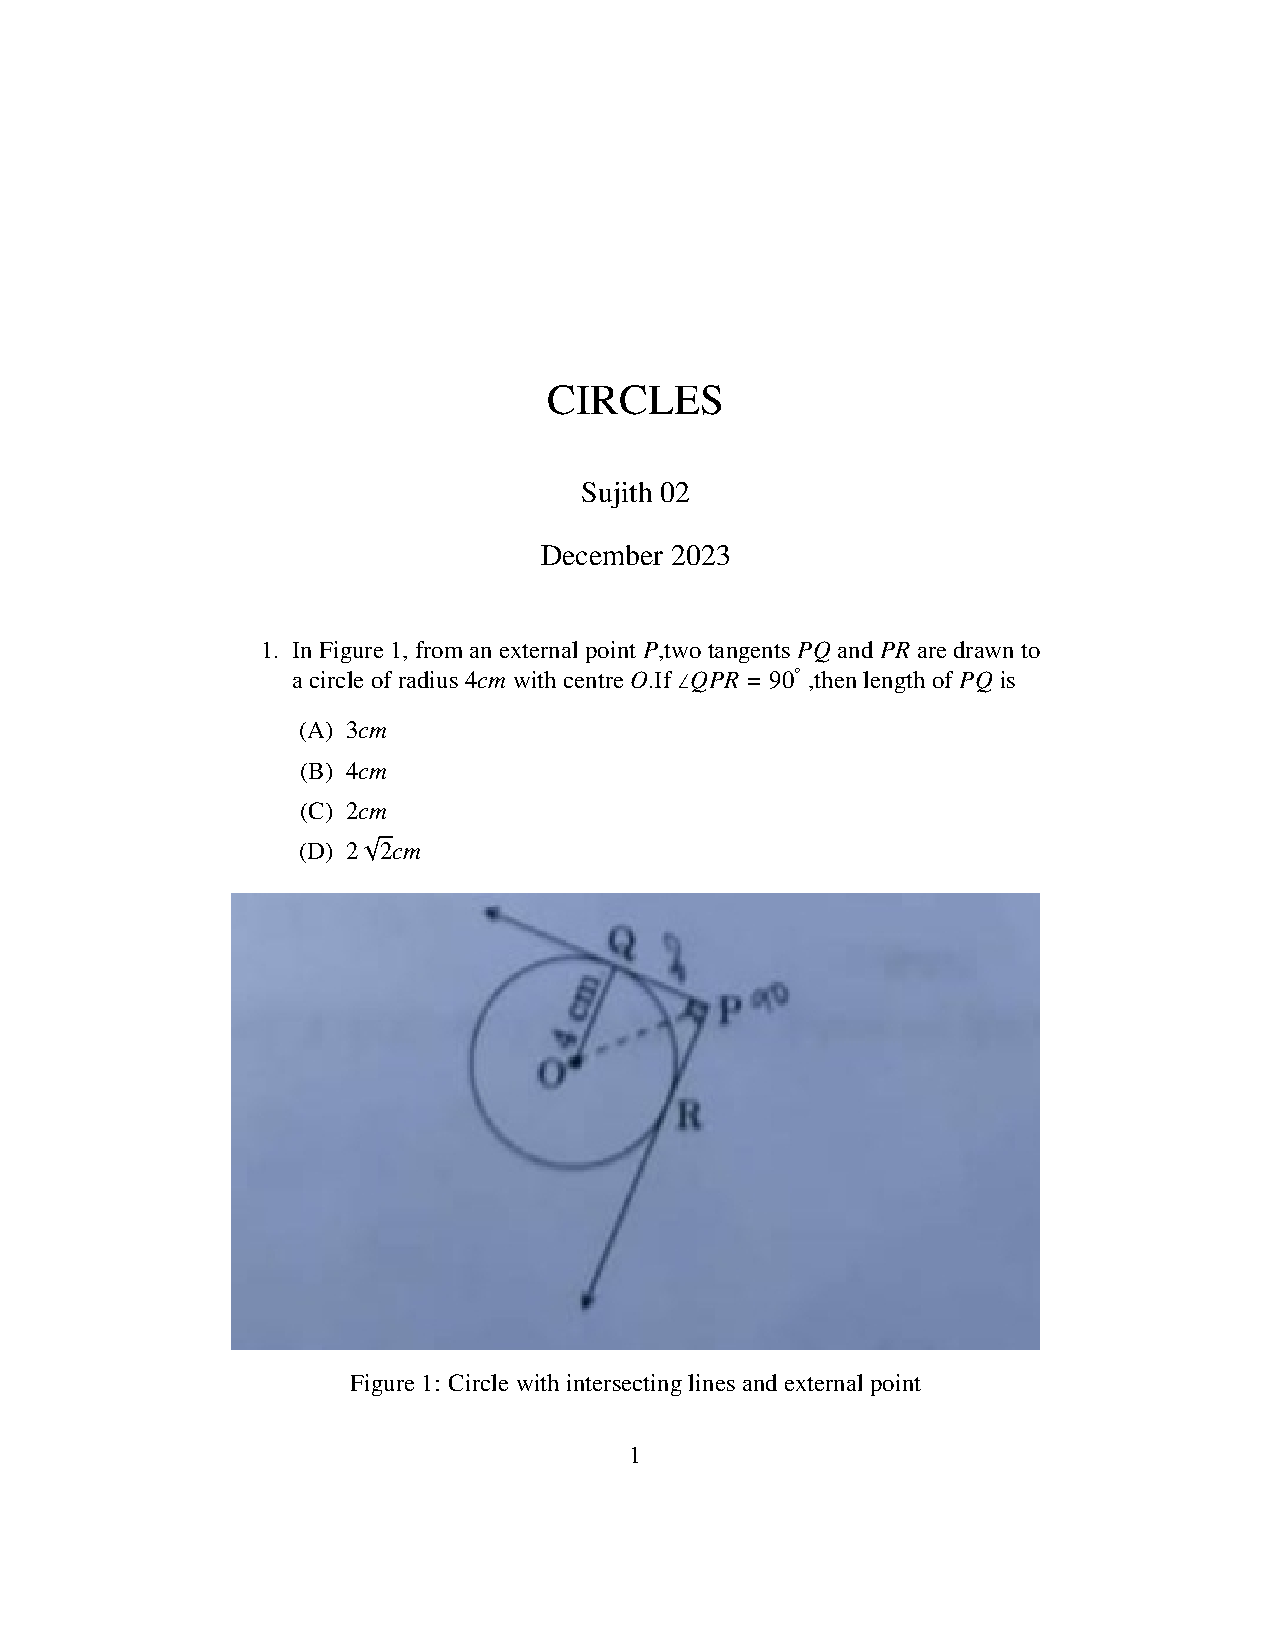
\includegraphics[width=\columnwidth]{figs/circ.jpg}
\caption{}
\label{fig:circ.jpg}
\end{figure}
\end{enumerate}
\item In \figref{fig:circ2.jpg}, $PQ$ is tangent to the circle with centre at $O$, at the point $B$. If $\angle AOB=100\degree$, then $\angle ABP$ is equal to
\begin{enumerate}[label=(\Alph*)]
\item $50\degree$
\item $40\degree$
\item $60\degree$
\item $80\degree$
\begin{figure}[H]
\centering                                       
\includegraphics[width=\columnwidth]{figs/circ2.jpg}  
\caption{}
\label{fig:circ2.jpg}                      
\end{figure}
\end{enumerate}
\item In \figref{fig:circ3.jpg}, a quardilateral $ABCD$ is drawn to circumscribe a circle.\newline Prove that \newline $AB+CD=BC+AD$.
\begin{figure}[H]
\centering
\includegraphics[width=\columnwidth]{figs/circ3.jpg}
\caption{}
\label{fig:circ3.pjpg}
\end{figure}
\item In \figref{fig:circ4.jpg}, find the perimeter of$\triangle{ABC}$, if $AP=12$cm.
\begin{figure}[H]
\centering
\includegraphics[width=\columnwidth]{figs/circ4.jpg}
\caption{}
\label{fig:circ4.jpg}
\end{figure}
\end{enumerate}
\end{document}
